\section{系统测试}
\subsection{系统测试简介}

本系统主要采用单元测试和集成测试的方式。

\subsubsection{测试方法}

\paragraph{单元测试}

单元测试又称为模块测试,是针对程序模块(软件设计的最小单位)
来进行正确性检验的测试工作。程序单元是应用的最小可测试部件。
在过程化编程中,一个单元就是单个程序、函数、过程等;
对于面向对象编程,最小单元就是方法,包括基类(超类)、抽象类、或者派生类(子类)中的方法。

\begin{figure}[hbt]
	
\includegraphics[scale=.5]{unittest.png}
	\caption{单元测试}
\end{figure}

\paragraph{集成测试}
集成测试又称组装测试,即对程序模块采用一次性或增值方式组装起来,
对系统的接口进行正确性检验的测试工作。
整合测试一般在单元测试之后、系统测试之前进行。
实践表明,有时模块虽然可以单独工作,但是并不能保证组装起来也可以同时工作。

本系统中,最需要测试的是词法分析器和语法分析器,保证词法分析器正确,语法分析器
才能正确工作;而保证语法分析器正确,才能使得后面的系统正确工作。

Catch2是一个开源的C++测试框架,它具有轻量、易用、扩展性强、模块化程度高等特点,
非常适合这个编译器系统。

\paragraph{测试覆盖度}

测试的目的是为了减少程序在运行时发生错误的可能,因此,一个重要的指标便是测试覆盖度。
它指在测试中运行的代码占总代码的比例,显然,如果测试覆盖度达到100\%左右,
就可以证明代码可以完全按照程序员的设想运行。

\paragraph{gcov}

gcov是源代码覆盖率分析和按语句分析的工具。
gcov生成程序中每个语句执行次数的精确计数,
并注释源代码,可以通过查看注释来查看分析结果。

gcov实用程序提供有关程序执行代码段的频率的信息。
它产生源文件的副本,并带有执行频率。
gcov实用程序不会产生任何基于时间的数据,并且仅适用于使用GCC套件编译的代码。

\paragraph{lcov}

lcov是GCC覆盖率测试工具gcov的图形化前端。
它收集多个源文件的gcov数据,
并创建包含带有覆盖率信息注释的源代码的HTML页面。
它还添加了概述页面,以便在文件结构中轻松导航。

\begin{figure}[hbt]
  \centering
  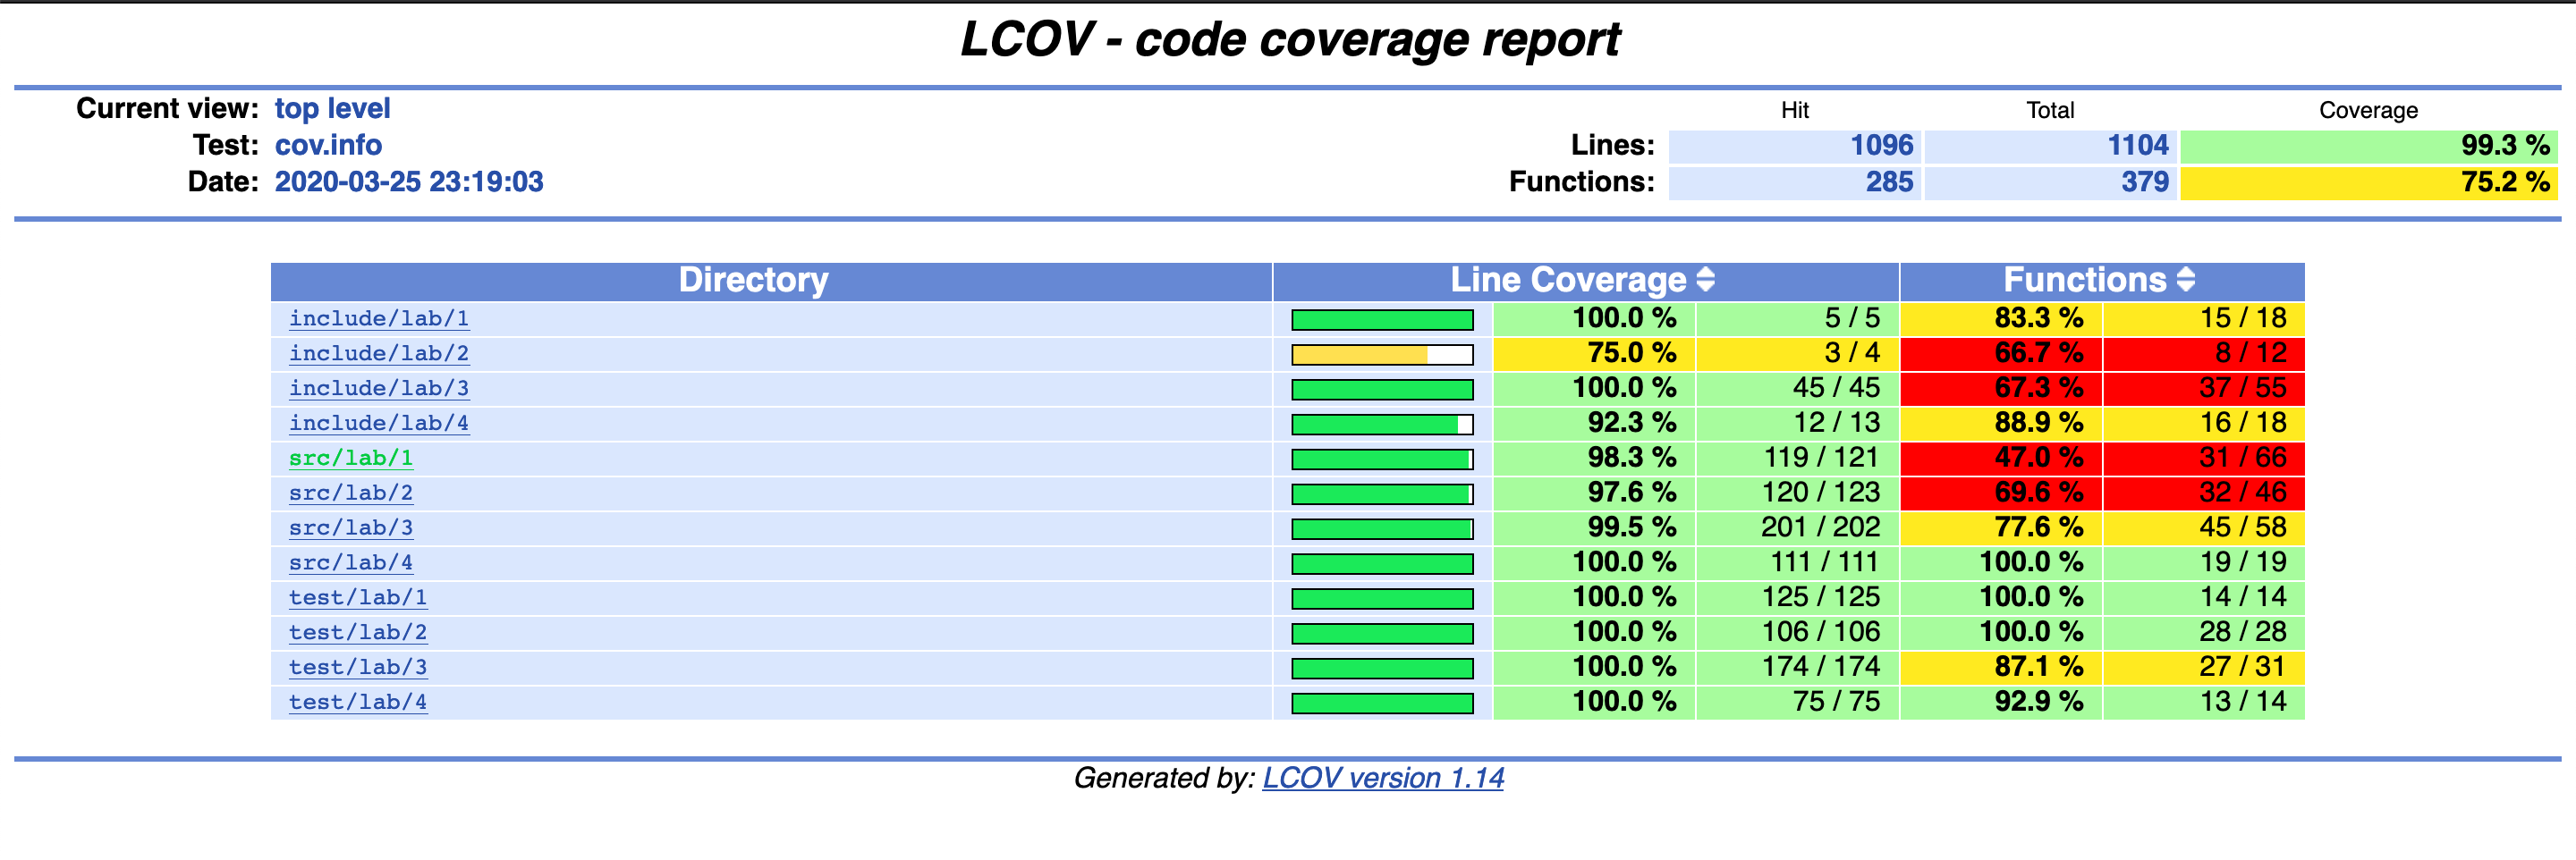
\includegraphics[scale=.3]{lcov.png}
  \caption{lcov界面}
\end{figure}

\subsection{系统单元测试}

\subsubsection{单元测试目标及数据选取}

\paragraph{词法分析器测试}

正如\autoref{sec:alldesign}中所说的,词法分析器需要做到正确判定每个标记的类别。
例如,\mintinline{cpp}|0xff, 123|等为数字,\mintinline{cpp}|int, void, for|等为关键字。
因此,我们用一些字符,用词法分析器来分析它,并判断得出的类型是否与预期相同。

此外,词法分析器还应该能做到适应任何数量、任何种类的分隔符。我们也要针对此做一些测试。
比如在两个标记中间添加若干不同种类的分隔符,检查词法分析器是否能正确识别。

除了正确性分析外,我们还需要给出一些不正确的标记,例如{\tt 0abc}。词法分析器需要
正确识别该标记的不合法性,并给出必要的提示。

\paragraph{语法分析器测试}

语法分析器的测试方法与词法分析器类似,首先是正确性分析,给出一定的正确语句,
通过语法分析器分析它,查看结果是否与预期相同。

同时,也需要进行错误测试,检查语法分析器能否正确识别并处理错误。

\subsubsection{测试大纲}

因为需要进行的测试比较多,因此使用JSON文件编写测试用例以及预期结果,
然后测试时将其读入并进行反序列化,然后分别运行测试。
完整的测试用例见\autoref{ch:test}。

\begin{listing}[hbt]
\begin{minted}{json}
[
  {
    "input": "0xff",
    "want": "Num",
  },
  {
    "input": "13",
    "want": "Num",
  },
  {
    "input": "for",
    "want": "For",
  },
  {
    "input": "\n",
    "want": "NewLine",
  },
]
\end{minted}
\caption{测试用例示例}
\end{listing}

\subsection{系统集成测试}

\paragraph{正确性测试}
集成测试则是需要将之前以及进行过单元测试的模块合起来一起测试,主要检测的是模块
间的接口是否对接成功。
由于我们使用的是递归下降的分析方式,如\autoref{sec:algorithm}所述,
词法分析器和语法分析器之间的耦合程度比较高,因此集成测试的意义并不大。
而自动化测试并不能对语法树打印器与代码生成器的结果进行比较好的测试,
所以我在集成测试中的正确性测试部分就没有采用自动化测试的方式,而是通过手动测试,
判断整个系统的输出是否与预期相同。

\paragraph{错误处理测试}
而在错误处理测试中,我同样给出若干存在问题的源文件,并通过JSON文件配置文件名及预期输出,
然后通过自动化工具进行测试。

\begin{listing}[hbt]
\begin{minted}{json}
[
  {
    "input": "e_for.c",
    "error": "expr error",
  },
  {
    "input": "e_while",
    "error": "stmt error",
  },
]
\end{minted}
\caption{测试用例示例}
\end{listing}

\subsection{测试结果}
% end
